\begin{section}{Aim of the Thesis}
Many studies on polythiophenes bearing chiral side groups are already present in the literature. 
There are also many articles on diblock copolymers with an achiral thiophenic block and a poly\-(vinyl\-pyridine) block.\superfootcite{Lohwasser2012}\superfootcite{Sary2010a}\superfootcite{Palaniappan2011}\superfootcite{Mougnier2012} In the literature we found also block copolymers made of two polythiophene blocks, one of these being chiral.\superfootcite{VandenBergh2010}\superfootcite{VandenBergh2008}\superfootcite{Verswyvel2011}\superfootcite{Verswyvel2013} A few articles on alternating block copolymers with chirality on the non thiophenic block can be found.\superfootcite{Henze2003} The aim of this thesis is to synthesize and study a polythiophene with a novel chiral side group and its use with a non chiral poly(4-vinyl\-pyridine) block in a diblock copolymer unreported in the literature. 
A modification of the optical activity of the di\-block copolymer with respect to that of polythiophene homo\-polymer could envisage a possible use of this material as a chiral probe in the aggregation process of bulk hetero\-junction solar cells fabricated using block copolymers as active layer.

Thus we started synthesizing a semiconductor, light harvesting chiral polymer with low polydispersity. Then, using an original convenient strategy, we functionalized a termination of the chiral polythiophene with an initiator for the living \gls{NMRP}, finally we polymerized a second block of poly\-(4-vinyl\-pyridine). The obtained diblock copolymer can be used in various devices like solar photovoltaic cells and in studies on supramolecular chirality.

\end{section}
\begin{section}{Introduction to Synthesis and Characterization}

\begin{subsection}{Monomer and Lateral Chains}

\paragraph{Oxygenated side chain} In order to synthesize a chiral polythiophene a monomer bearing a chiral side chain was used. Many different side chains and monomers could fit our requirements. The source of chirality was chosen as an inexpensive and non toxic\superfootcite{McGinty2010} chiral alcohol: (S)-2-methyl-1-butanol also known as active amyl alcohol, present in nature as a component of fusel alcohol which is a by-product of alcoholic fermentation. Our syntheses produced polythiophenes with a (2-methyl\-butyl\-oxy)\-methyl side chain which is, to the best of our knowledge, unreported in the literature. 
Due to the presence of an oxygen atom in the side chain, electronic levels (\acrshort{HOMO} and \acrshort{LUMO}) of the resulting polythiophenes will be different from electronic levels of the well known \gls{P3HT}.\superfootcite{VanBeek2005}\superfootcite{McCullough1993}\superfootcite{Daoust1991} 
The length of the side chain was chosen to be short enough to allow a good charge mobility in a future material for organic electronics.

\paragraph{Enantiomeric excess} For studying the importance of chirality we synthesized two monomers with different enantiomeric excesses: an enantiopure monomer and a scalemic\nota{\textit{scalemic}, non racemic.}
one having 59~\% optical purity.\nota{\label{fn:opticalpurity}\textit{optical purity}, the ratio of the observed optical rotation of a sample consisting of a mixture of enantiomers to the optical rotation of one pure enantiomer. (IUPAC Gold Book)} We used a scalemic alcohol due to the unavailability of the racemate. 

\end{subsection}
\begin{subsection}{Regioselectivity of Monomer Activation}

\paragraph{Grignard activation} The activation process, which is the first step of the polymerization method, consists in a metalation in position 5 of thiophene ring (see Figure~\ref{fig:regioregolarita} for position numbering). As stated in page~\pageref{intro-polimerizzazione}, both zinc
(Rieke method) and magnesium (McCullough method) can be used for this aim. The latter is the most commonly used because allows a more controlled polymerization,\superfootcite{Sheina2004}\superfootcite{Iovu2005}\superfootcite{Yokoyama2004}\superfootcite{Miyakoshi2005} thus we activated our monomer as a Grignard reagent. 
The metalation on iodine was performed with a Grignard metathesis\nota{\textit{metathesis}, a bimolecular process formally involving the exchange of a bond (or bonds) between similar interacting chemical species so that the bonding affiliations in the products are identical (or closely similar) to those in the reactants. (IUPAC Gold Book)} 
(\acrshort{GRIM}), a reaction of replacement of a halogen atom by a metal from an organometallic compound.\superfootcite{Knochel2003}\superfootcite{Tamborski1971}\superfootcite{Zakharkin1964} 
Both Grignard formation\superfootcite{Krasovskiy2004}\superfootcite{Hauk2006} and subsequent polymerization\superfootcite{Takahashi2010}\superfootcite{Lohwasser2011}\superfootcite{Miyakoshi2006}\superfootcite{Ono2012}\superfootcite{Lanni2009}\superfootcite{Lanni2010} are facilitated by the addition of lithium chloride, but the resulting polymers could have lower regioregularity.\superfootcite{Lohwasser2011} 
Tert-butyl magnesium chloride and iso-propyl magnesium chloride are the most common activating Grignard reagents, the former could give a slightly better selectivity\superfootcite{Loewe2001} towards the less sterically demanding 5 position, but iso-propyl magnesium chloride is reported to be sufficiently regioselective when a iodine-bromine monomer is used.\superfootcite{Takahashi2010}\superfootcite{Lohwasser2011}\superfootcite{Ono2012} 
Iso-propyl magnesium chloride could lead to iso-propyl terminated polymers,\superfootcite{Kiriy2011}\superfootcite{Jeffries-EL2004}\superfootcite{Lohwasser2011}\superfootcite{Miyakoshi2005} this eventuality will be verified by Matrix-assisted laser desorption ionization\nota{\textit{matrix-assisted laser desorption ionization}, 
a soft ionization technique used in mass spectrometry, allowing the analysis of large organic molecules. (Wikipedia)}--time-of-flight mass spectrometry.\nota{\textit{time-of-flight mass spectrometry} or TOF MS, is a method of mass spectrometry in which an ion's mass-to-charge ratio is determined via a time measurement. (Wikipedia)}

\begin{SCfigure}[][tbp]%gaussian-grignard
\centering
\begin{subfigure}[b]{0.35\textwidth}
\centering
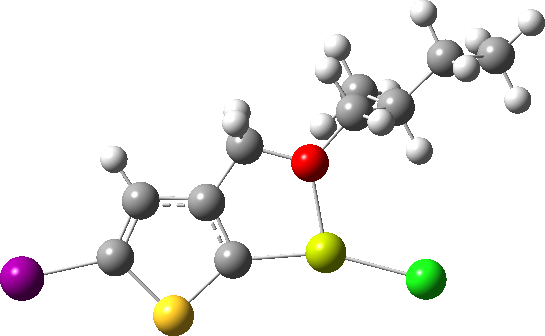
\includegraphics[width=\textwidth]{gaussian-grignard-2.png}
\subcaption{}
\label{fig:gaussian-grignard-2}
\end{subfigure}%
~%add desired spacing between images, e. g. ~, \quad, \qquad etc.
%(or a blank line to force the subfigure onto a new line)
\begin{subfigure}[b]{0.28\textwidth}
\centering
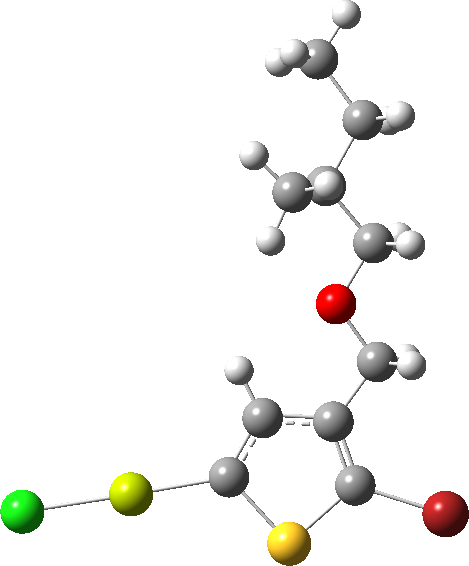
\includegraphics[width=\textwidth]{gaussian-grignard-5.png}
\caption{}
\label{fig:gaussian-grignard-5}
\end{subfigure}
\caption[Activated monomers.]{Activated monomers. (\subref{fig:gaussian-grignard-2}) Grignard formation in position 2, \ch{MgCl} substitutes \ch{Br}.\\ (\subref{fig:gaussian-grignard-5}) Grignard formation in position 5, \ch{MgCl} substitutes \ch{I} (optimization Gaussian\-09c01\-/DFT\-/B3LYP\-/LanL2DZ).}\label{fig:gaussian-grignard}
\end{SCfigure}

\paragraph{Influence of side chain on activation} In the case of a thiophene monomer with an alkyl side chain the steric effect by the side group is sufficient to obtain 85 \% regioselectivity even using a dibromide monomer.\superfootcite{Loewe2001}\superfootcite{Iovu2005}\superfootcite{Chen1993} 
But when an oxy\-methylene side group is present, using a dibromide monomer leads to regiorandom polymers\superfootcite{Ohshimizu2008}\superfootcite{Zoombelt2008} while using a iodide-bromide monomer leads to regioregular polymers.\superfootcite{Ohshimizu2008}\superfootcite{Zoombelt2008}\superfootcite{Adachi2006}\superfootcite{Locke2010} 
We suppose that this lack of regioselectivity is related to the formation a five-member ring with the oxygen atom coordinating the magnesium atom in position 2, as shown in Figure~\ref{fig:gaussian-grignard-2}, therefore favoring the formation of the undesired 2-magnesio\-chloro-5-iodo-3-[((S)-2-methyl\-butyl\-oxy)\-methyl]\-thio\-phene. This ring formation can't take place with the product of \gls{GRIM} in position 5, as shown in Figure~\ref{fig:gaussian-grignard-5}, with 2-bromo-5-magnesio\-chloro-3-[((S)-2-methyl\-butyl\-oxy)\-methyl]\-thio\-phene.

\end{subsection}
\begin{subsection}{Polymerization Regioregularity}

\begin{SCfigure}[][tbp]%regioregolarita
\centering
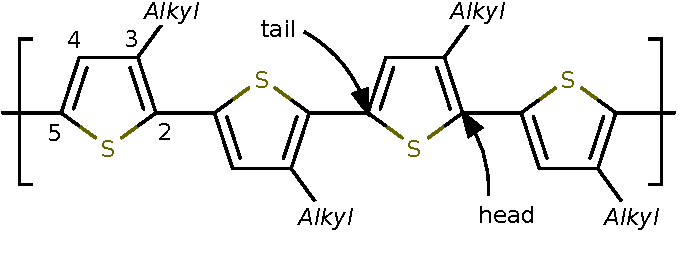
\includegraphics[scale=0.7]
{regioregolarita.pdf}
\caption{Regioregular poly-3-alkylthiophene, \textit{head-to-tail} and numbered thiophene positions.}
\label{fig:regioregolarita}
\end{SCfigure}

\paragraph{Importance of regioregularity} In order to obtain a solar light harvesting and semiconducting polymer we chose to synthesize a regioregularly substituted conjugated polythiophene. The substitution with flexible side chains is necessary to process the otherwise insoluble and infusible unsubstituted polythiophene. Undoped polythiophenes usually absorbs the high energy portion of the solar radiation spectrum, thus a red shift in absorption is welcomed and can be obtained by a reduction of the band gap. 
As stated earlier the band gap width is related both to the electronic molecular properties of the side group and to the extension of conjugation along the polymer. This in turn depends on the coplanarity of the aromatic rings that is avoided by repulsion between side groups. 
In conclusion we want to polymerize a thiophene bearing a single side chain in a regioregular\nota{\label{fn:regioregular}\textit{regioregular}, a polymer in which each repeat unit is derived from the same isomer of the monomer. (Wiktionary)}\superfootcite{Kim2006} 
repetition so that the distance between side chains is maximized and no backbone twist is induced by steric repulsions. As indicated in Figure~\ref{fig:triadi}, a way of referring to the relative orientation of two monomeric units is \textit{head-to-head}, \textit{tail-to-tail} or \textit{head-to-tail}, meaning that the \textit{head} of a monomer, the position 2, nearest to the side chain, or the \textit{tail}, the position 5, farthest from the side group, is directly bonded to the \textit{head} or the \textit{tail} of the successive monomer. 
An ordered planar conformation and tight interdigitation in aggregates can be obtained only with a \textit{head-to-tail} polythiophene, thus a good regioregularity is of crucial importance for aggregation and morphology,\superfootcite{Samitsu2008}\superfootcite{Samitsu2008a}\superfootcite{Goto2000}\superfootcite{Goto2002}\superfootcite{McCullough1993c}\superfootcite{McCullogh1995}\superfootcite{Adachi2011}\superfootcite{Xu1993} but it is also important for intra-chain conduction\superfootcite{Basescu1987} and is necessary for supramolecular expression of side chains chirality.\superfootcite{Bouman1994a} 

\begin{SCfigure}[][tbp]%triadi
\centering
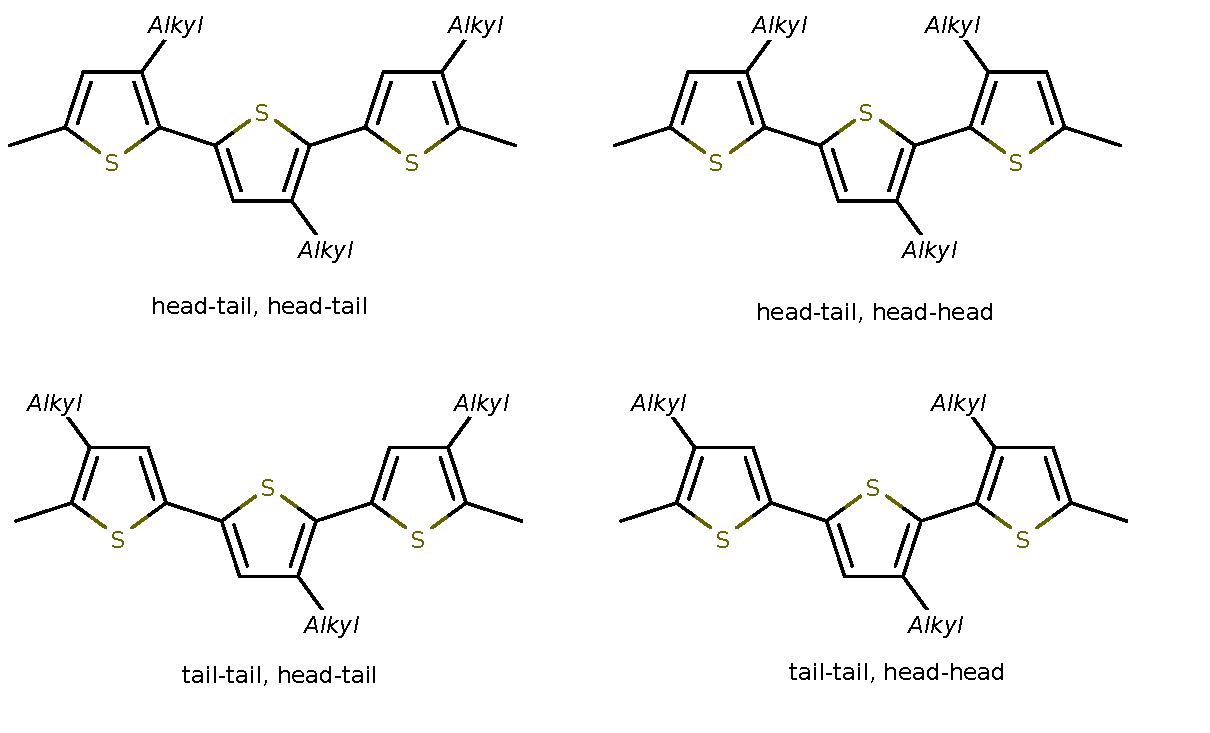
\includegraphics[scale=0.6]
{triadi.pdf}
\caption{Possible triads of monosubstituted thiophene rings.}
\label{fig:triadi}
\end{SCfigure}

\begin{figure}[tbp]%iniziazione-meccanismo
\centering
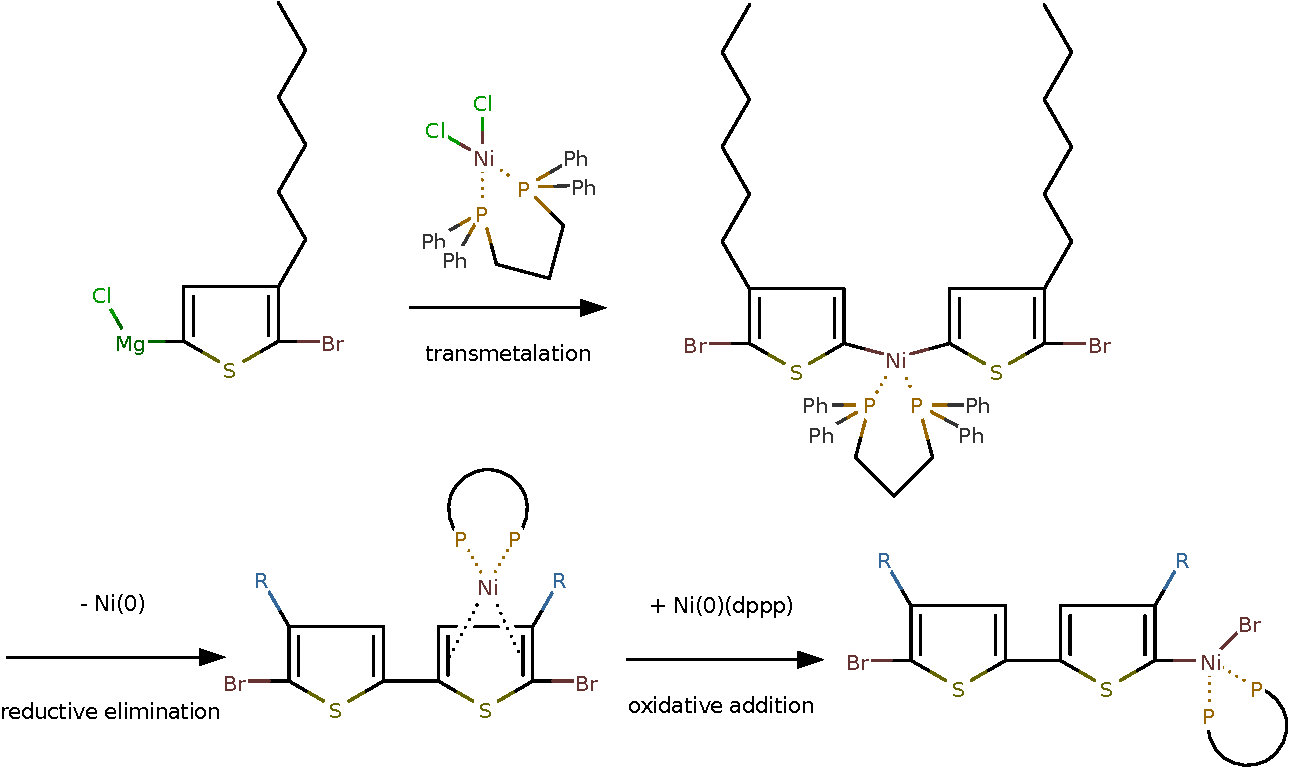
\includegraphics[width=1\textwidth]
{iniziazione-meccanismo.pdf}
\caption{Mechanism of initiation in nickel catalyzed dehalogenative polycondensation.}
\label{fig:iniziazione-meccanismo}
\end{figure} 

\paragraph{Obtaining regioregularity} Regiocontrolled polymerization of thiophene can be achieved with nickel catalyzed dehalogenative polycondensation\nota{\label{fn:polycondensation}\textit{condensation polymer}, the molecular formula of the monomer differs from that of the structural unit. %(\citeauthor*{Carothers1929}\superfootcite{Carothers1929})
} 
starting from a regioselectively activated monomer.\superfootcite{Chen1992}\superfootcite{Chen1995}\superfootcite{McCullough1993a}\superfootcite{Loewe2001}\superfootcite{Loewe1999}\superfootcite{Mao2004}\superfootcite{McCullogh1995}\superfootcite{McCullough1993c} 
This method produces a polymer with high regioregularity even in presence of some monomer activated in the \textit{wrong} position.\superfootcite{Chen1995}\superfootcite{Loewe2001}\superfootcite{Iovu2005}\superfootcite{Lanni2010}\superfootcite{Lohwasser2011} 
The initiation mechanism is illustrated for \acrfull{P3HT} in Figure~\ref{fig:iniziazione-meccanismo}. Initially a transmetalation occurs, two magnesium atoms on two activated thiophenic units are exchanged with the nickel(II) atom of the catalyst. Then a reductive elimination produces a nickel(0) complex and a symmetric dimer that will be present in a chain extremity as a \textit{tail-to-tail} dyad, a defect in regioregularity.\superfootcite{Verswyvel2011}\superfootcite{Tkachov2010}\superfootcite{Miyakoshi2005} 
At this point the nickel(0) complex can perform an oxidative addition in a thiophenic \ch{C-Br} bond starting the propagation stage.
Then, as shown in Figure~\ref{fig:regioregolarita-meccanismo}, on the \ch{CNi-Br} bond a transmetalation occurs (or, from the nickel point of view, an exchange in anions) involving an activated monomer. A subsequent reductive elimination and oxidative addition complete the propagation mechanism. 
The use of a nickel catalyst, rather than a palladium one, and the use of a chelating ligand with wide bite angle are essential conditions for obtaining a good regioselectivity.\superfootcite{Chen1995}\superfootcite{Choi2010}\superfootcite{Mao2004} Indeed we used \acrlong{nidppp} (\acrshort{nidppp}, \acrshort{dppp} = \ch{Ph2P(CH2)3PPh2}) which is the most widely utilized catalyst for regioregular nickel catalyzed dehalogenative polycondensation.

\begin{figure}[tbp]%regioregolarita-meccanismo
\centering
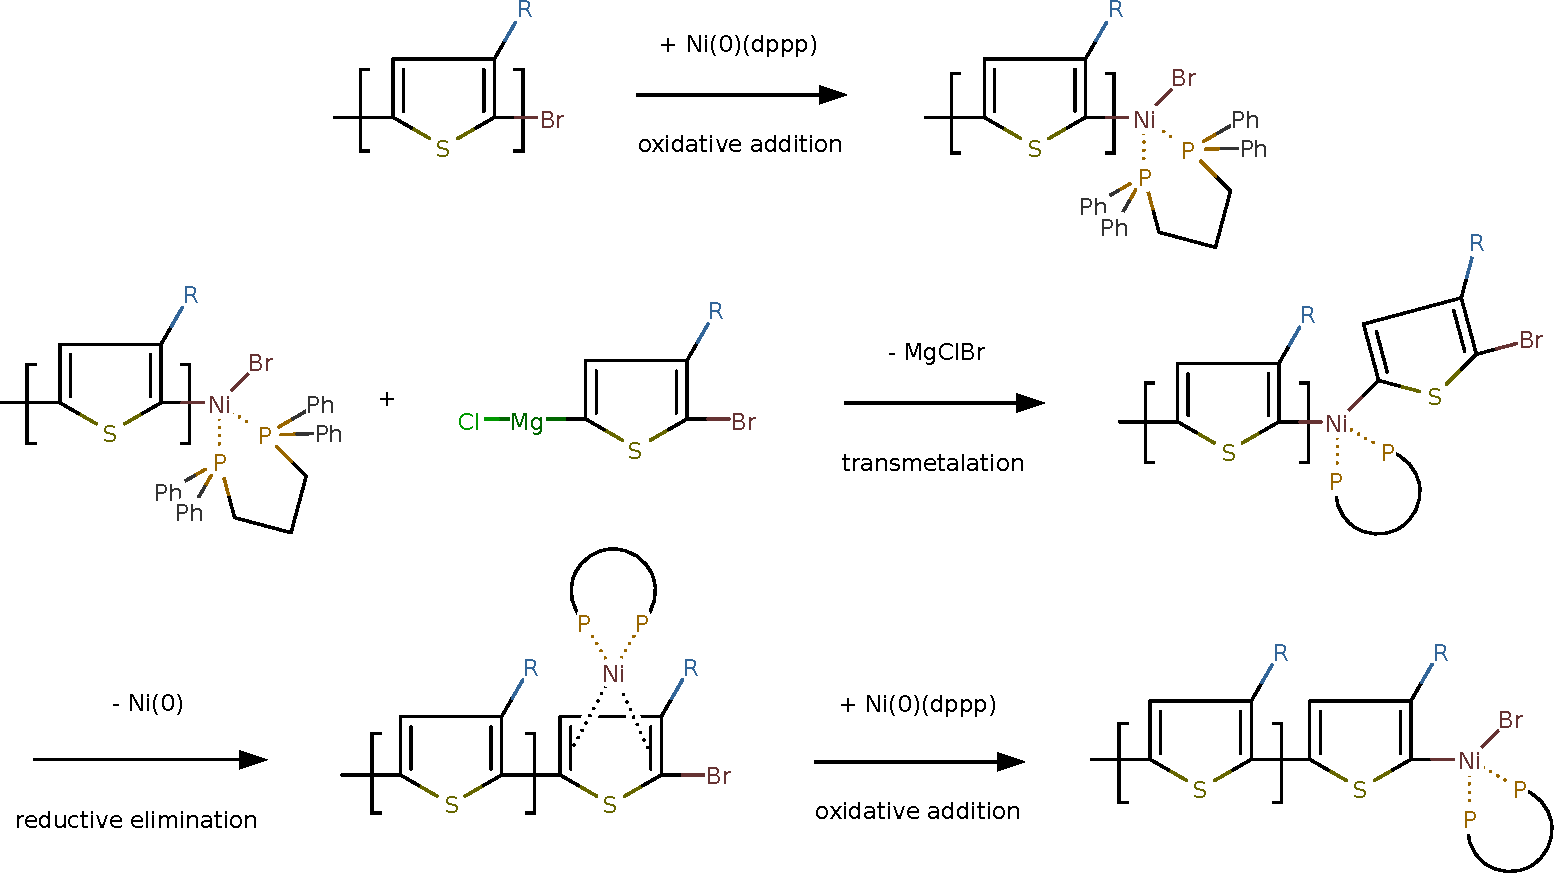
\includegraphics[width=1\textwidth]
{regioregolarita-meccanismo.pdf}
\caption{Mechanism of propagation in nickel catalyzed dehalogenative polycondensation.}
\label{fig:regioregolarita-meccanismo}
\end{figure} 

\paragraph{Evaluating regioregularity} The regioregularity can be qualitatively evaluated by absorption in solution\superfootcite{Chen1995}\superfootcite{McCullough1993c} and quantitatively by \gls{NMR}.\superfootcite{Jeffries-El2005}\superfootcite{Chen1995}\superfootcite{Chen1992}\superfootcite{Zoombelt2008}\superfootcite{Maior1990}\superfootcite{McCullough1993c}
With our uncommon polythiophenes, evaluating the regioregularity from absorption maxima in chloroform solution is not feasible because of the variance of the data reported in the literature.\superfootcite{Higashihara2011}\superfootcite{VanBeek2005}\superfootcite{Ohshimizu2008}\superfootcite{McCullough1993}\superfootcite{Zoombelt2008}\superfootcite{Saito2005}\superfootcite{Locke2010}\superfootcite{Bouman1994} 
At {\HNMR} the aromatic hydrogen peak and the $\alpha$-methylenic peak of a thiophenic unit are influenced by the orientations of nearby repeating units, giving a different peak for each situation showed in Figure~\ref{fig:triadi}. In our case the signals arising from each situation are singlets from both aromatic and aliphatic protons, thus it's easy to distinguish the presence of nearby signals. This is an advantage over \gls{P3HT} in which the peak from the first methylene in the aliphatic side chain is a triplet. 

\end{subsection}
\begin{subsection}{Polymer Weight Control}

\paragraph{Block copolymers} 
As seen in Section~\ref{intro-pv}, 
to stabilize a \acrfull{BHJ} structure (see Figure~\ref{fig:bhj}) against segregation a possible approach is to use block copolymers as compatibilizer or as main component.\superfootcite{Topham2011} In this thesis we'll synthesize an amphiphilic diblock copolymer poly\-thio\-phene-poly\-(4-vinyl\-pyridine). 
The polythiophene block acts as \textit{p}-type material, electron donor. The poly\-(4-vinyl\-pyridine) doesn't act itself as electron acceptor, indeed it complexes modified fullerenes (usually \acrlong{PCBM}, \acrshort{PCBM}, but also non functionalized fullerene\superfootcite{Laiho2006}) which act as \textit{n}-type semiconductor. The optimization of relative volume fraction of the polymer blocks can produce a bicontinuous interpenetrating network of donor and acceptor materials that would give a better charge mobility.

\paragraph{Importance of weight} A low polydispersity helps the crystallization process, thus helping the polymer to give a high interchain charge mobility. Polydispersity is important also for the aggregation morphology of block polymers.\superfootcite{Maria2008}\superfootcite{Koningsveld1972}\superfootcite{Hong1981}\superfootcite{Whitmore1985} Controlling the molecular weight of the polymer is important in this system because changing block dimension can lead to a different blend morphology.\superfootcite{Topham2011} 
Moreover it is important in rod (rigid, conjugated along the backbone) polymers due to their incapacity of chain stretching to accommodate packing of a statistical distribution of chain sizes within an uniformly sized nano\-domain. In brief, high polydispersity could disturb the crystallization needed for a good charge transportation and introduce disorder in the formation of complex morphologies in block copolymers.\superfootcite{Schlaad2004}

\paragraph{Polymerization mechanism} \label{kctp} Most of the conducting conjugated polymers are synthesized by step-growth\nota{\textit{step-growth polymerization}, a polymerization mechanism where any termination on growing oligomers or monomers can react with any other terminations.} poly\-condensation\superfootcite{conj-sint} resulting in high polydispersity polymers. 
In 2004 a quasi-living\nota{\textit{living polymerization}, a chain polymerization from which chain transfer and chain termination are absent. In many cases, the rate of chain initiation is fast compared with the rate of chain propagation, thus that the number of kinetic-chain carriers is essentially constant throughout the polymerization. (IUPAC Gold Book)} 
chain-growth\nota{\label{fn:chain-growth}\textit{chain-growth polymerization}, a polymerization technique where unsaturated monomer molecules add onto the active site on a growing polymer chain one at a time. Growth of the polymer occurs only at one (or possibly more) ends. Addition of each monomer unit regenerates the active site. (Wikipedia)} 
mechanism was reported\superfootcite{Yokoyama2004}\superfootcite{Sheina2004} for nickel catalyzed de\-halogenative polycondensation of \acrfull{P3HT}. 
The chain-growth character is possible thanks to the loose coordination of \ch{Ni}(0) on the growing polythiophene chain forming a non-diffusive associated pair (as illustrated in Figures~\ref{fig:iniziazione-meccanismo} and \ref{fig:regioregolarita-meccanismo}), thus the oxidative insertion step can occur only in a \ch{C-Br} bond on the growing chain.\superfootcite{Tkachov2010}\superfootcite{Zenkina2008}\superfootcite{Miyakoshi2005}\superfootcite{Jeffries-El2005}\superfootcite{Tkachov2010}\superfootcite{Sheina2004} This recent polymerization method is named \gls{KCTP}. 
Up to now it was extended to a few other polymers different from polythiophene while maintaining a living character.\superfootcite{Ono2012}\superfootcite{Wu2010}\superfootcite{Yokoyama2008} Obviously the catalyst is important and again \gls{nidppp} resulted as the best performing for living poly\-merizations of poly(3-alkyl\-thio\-phenes).\superfootcite{Choi2010}\superfootcite{Senkovskyy2009}\superfootcite{Bronstein2009}

\paragraph{Second block polymerization} \Acrfull{P4VP} was chosen as the polar component in our amphiphilic block copolymer. Various block copolymer with a complexing \acrshort{P4VP} block are already present in the literature.\superfootcite{Sary2010a}\superfootcite{Lohwasser2012}\superfootcite{Palaniappan2011}\superfootcite{Mougnier2012}\superfootcite{Laiho2006}\superfootcite{Maria2008}\superfootcite{Sun2011} The molecular weight of the coil (not rigid) block is important too, thus a living polymerization was used: the chain-growth living \acrfull{NMRP}. 
In the present case we chose the grafting-from\nota{\textit{grafting-from polymerization}, the initiator for a polymerization is chemically bonded on a pre-existing polymer.} approach starting the polymerization of poly(4-vinyl\-pyridine) from a macroinitiator bonded on the end of the polythiophene chains. 
A grafting-onto\nota{\textit{grafting-onto polymerization}, two or more formed polymers are chemically joined to form a multi\-block polymer.} 
approach would have permitted a better characterization of the second block, but obtaining a diblock copolymer (rather than a triblock or more) would have required the asymmetric termination of both polymeric blocks. 
A further significant aspect to be taken into account using this approach is the chelating ability of poly(4-vinyl\-pyridine) that would disturb the joining process chelating any metal or catalyst needed for the reaction. 

\end{subsection}
\begin{subsection}{Polymer Terminations Control}
A chain-growth polymerization is the way to synthesize an asymmetrically terminated macroinitiator. Thankfully quasi-living Kumada catalyst-transfer polycondensation can give asymmetric termination of the polythiophene chains\superfootcite{Jeffries-El2005}\superfootcite{Lohwasser2011} and in the literature we can find many diblock copolymers synthesized with a combination of \gls{KCTP}--\gls{NMRP}.\superfootcite{Zhang2009}\superfootcite{Britze2011}\superfootcite{Kaul2010}\superfootcite{Mougnier2012}\superfootcite{Richard2008}

\paragraph{Polymerization quenching} The quenching process is reported to be crucial in order to obtain a quasi-mono\-dispersed polymer and defined terminations. 
Quenching simply with water\superfootcite{Miyakoshi2004} or methanol\superfootcite{Lohwasser2011} can cause dimerization via disproportionation of the poly\-thio\-phene--\ch{Ni}(0)--\ch{Br} complex, followed by reductive elimination of poly\-thio\-phene--poly\-thio\-phene with doubled weight. Quenching with aqueous hydrochloric acid is reported to prevent dimerization.\superfootcite{Miyakoshi2004}\superfootcite{Lohwasser2011} 
Quenching with certain Grignard reagents can even react \textit{in situ} with a single chain end to give asymmetrically functionalized poly\-thio\-phenes.\superfootcite{Jeffries-El2005}\superfootcite{Jeffries-EL2004} We preferred to quench with aqueous hydrochloric acid because it promised for a reliable \ch{H/Br} termination.\superfootcite{Lohwasser2011}

\end{subsection}
\begin{subsection}{Optical Properties}
\paragraph{Band gap} We expect a polythiophene with a rather usual band gap energy (\SI{\approx1.9}{\eV}) but a slightly different \gls{LUMO} 
energy and \gls{HOMO} energy. 
These energy levels are an essential parameter of thin film photovoltaic devices,\superfootcite{Scharber2006}\superfootcite{Cremer2006}\superfootcite{Koster2006} in fact it is well known that open circuit voltage ($\mathrm{V_{oc}}$, which is a generally accepted estimate for the built-in potential) has an upper limit derived from the difference between \gls{HOMO} of the electron donor material and \gls{LUMO} of the electron acceptor material.\superfootcite{Brabec2001}\superfootcite{Gadisa2004} An electron withdrawing substituent in the donor material could move the electronic levels increasing the oxidation potential, this would increase the $\mathrm{V_{oc}}$. 
In the literature on polythiophenes the presence of a \ch{-CH2-O-R} side group is reported as beneficial for various photovoltaic devices\superfootcite{VanBeek2005}\superfootcite{Zoombelt2008} and for the conducting properties of materials.\superfootcite{Bryce1987} 

\paragraph{UV-vis} 
The study of solvato\-chromism reveals the formation of aggregates and the aggregation quality. Both an interaction of chains giving an exciton coupling and an extension of the conjugation length, result in a red-shift of the \gls{UVvis} absorption peak. When a certain amount of non-solvent is added to a solution of polymer, aggregation occurs giving a colloidal dispersion. The conditions for obtaining an aggregate can deeply influence the resulting morphology.\superfootcite{Kiriy2003}\superfootcite{Kim2010}\superfootcite{Goto2002}\superfootcite{Salatelli2010} 
In order to verify the solid state aggregation and morphology, we employed various sample preparation methods: spin coating, drop casting and dispersion in \ch{KCl} disk. 

These three methods should allow us to obtain different semi\-crystallinity extents: spin coating should avoid an organization of polymer chains, drop casting produces both an amorphous mixed with a crystalline solid, \ch{KCl} disks preparation employs dry polymer, thus should result in the most well packed structure. The presence of a vibronic fine structure suggests, but don't assure, the presence of some crystalline domains in the material.

\end{subsection}
\begin{subsection}{Photoluminescence and Chirality}
\paragraph{Photoluminescence} One of the aims of introducing chirality in our polymer was to influence the aggregation morphology, avoiding a parallel chain stacking, in order to reduce exciton quenching related to inter chain coupling. We suppose that studying photoluminescence quenching can help us to understand also exciton quenching.\superfootcite{Theander1999}\superfootcite{Kaneto1989} It was already reported that an aggregation morphology in which chains adopt a non parallel relative orientation results in highly fluorescent materials.\superfootcite{Zahn2002}\superfootcite{Deans2000}%
\superfootcite{Bredas1999}

\paragraph{Chirality as a probe} Talking of bulk heterojunction solar cells we are referring to soft-matter, quite disordered, difficult to characterize in the solid state. As stated in page~\pageref{intro-cd}, introducing some extent of chirality in our material allows us to use circular dichroism spectroscopy to characterize also aggregated states. 
In an assembly with chirally oriented identical transition dipole moments in close spatial proximity, their interaction brings about a splitting, called Davydov splitting,\nota{\textit{Davydov splitting}, the splitting of bands in the electronic or vibrational spectra of crystals due to the presence of more than one (interacting) equivalent molecular entity in the unit cell. (IUPAC Gold Book)} %
which is reflected in two distinct \gls{CD} bands 
with opposite rotational strength.\superfootcite{Berova2007} 
The sum of these two Cotton signals\nota{\label{fn:cottoneffect}\textit{Cotton effect}, the characteristic change in optical rotatory dispersion and/or circular dichroism in the vicinity of an absorption band of a substance. In a wavelength region where the light is absorbed, the absolute magnitude of the optical rotation at first varies rapidly with wavelength, crosses zero at absorption maxima and then again varies rapidly with wavelength but in opposite direction. (Wikipedia)} 
is a bisignate couplet. 
In polythiophenes the chromophore, for $\pi-\pi^*$ transitions, is located on the conjugated backbone. We can imagine the chromophore as a segment of the chain, as long as the conjugation length. Usually bisignate couplet signals arise from interchain interactions\superfootcite{Langeveld-Voss1999} but seldom also from intra-chain interactions.\superfootcite{Kiriy2003}\superfootcite{Nilsson2004}\superfootcite{Langeveld-Voss1996} The sign of the couplet can indicate the relative orientation of the chromophores.\superfootcite{Langeveld-Voss1998} 

\paragraph{Chirality in good solvent} Chiral polythiophenes in a good solvent usually exhibit only very weak electronic circular dichroism\superfootcite{Salatelli2010} because when the chain is well solvated chirality in side groups doesn't influence the $\pi-\pi^*$ transitions of the backbone. 

\paragraph{Chirality in poor solvent} When the conjugated chains interact with each other, the side groups rotational freedom is reduced and their chirality influences the organization of the material via steric repulsion. Adding a poor solvent or a non solvent to a solution of polymer, we can observe the rising of an induced circular dichroism during the formation of aggregated states; this can be caused by main chain twists or by a supramolecular chiral organization. 
The percent of non solvent can have a non trivial effect on the obtained aggregate\superfootcite{Bidan1996}\superfootcite{Goto2000} which can be studied via circular dichroism spectroscopy. Moreover changing solvent and/or non solvent could change dramatically the kind of aggregation and the \gls{CD} spectra of the supramolecular assembly.\superfootcite{Salatelli2010}\superfootcite{Goto2002}\superfootcite{Langeveld-Voss1998a} We employed mixtures of good and poor solvents like: chloroform-methanol, chloroform-acetonitrile, tetrahydrofuran-methanol and tetrahydrofuran-acetonitrile.

\end{subsection}
\end{section}